
\section{Ontology Usage}
\label{chap:usage}

% ontologie mohou dobre popsat openstack architekturu, protoze openstack vyuziva message bus, service catalog. Ontologie slouzi pak nad ramec openstack sluzeb u serveru ale definuji i vlastni operacni systemy a pridruzene sluzby - monitorting, metering, firewally, backupy, log management atd

The journey to mapping high level models in ontologies was long. It was a process of describing everchanging architectures of OpenStack cloud installations over past 2 years. The OpenStack released 4 major versions with 12 minor changes. The number of software components grew from 5 to 17. At the beginnings we started mapping meta-data models in separate files containing complete meta-data set of all services for each server or device. The meta-data was encoded in YAML format. This approach was manageable at earlier versions of OpenStack we tested and just the basic set of OpenStack services existed at the time. 

\begin{lstlisting}
service_name:
  service_role:
    data_parameter1: data_value1
    data_parameter2: data_value2
    data_parameter3:
    - data_value3a
    - data_value3b    
    object_parameter:
     object1:
       data_parameter1a: 
\end{lstlisting}


The next step was storing the service meta-data in hierarchical databases. The meta-data was split into components. 


All services  can be very well described by ontology as they communicate over common message bus, serialize their state and expose services through interfaces in a standard way. Nevertheless the optimal installations consist of at least following services.

All nodes providing contain basic set of

linux.system, linux.network, linux.storage - Basic configuration of network interfaces, users, volume, mounts, etc.

ntp.client - Time synchronisation is important when using common message bus

salt.minion/pupper.agent - Configuration management client provide

collectd.client, sensu.client - Monitoring services that provide common checks and meters for other services hosted on the same servers.

Controller node

mysql.cluster, rabbitmq.cluster, haproxy.proxy, corosync.cluster -

keystone.server, glance.server, nova.server, neutron.server, cinder.server, horizon.server - 

neutron.bridge -

Compute node

nova.compute, neutron.switch

\begin{figure}[!h]
\centering
\begin{lstlisting}
service_name:
  service_role:
    data_parameter1: data_value1
    data_parameter2: {service_name:service_role:data_paramer1}
    object_parameter:
     {otherobject:object1}
\end{lstlisting}
\caption{YAML encoded meta-data}
\label{fig:cm}
\end{figure}


% ontologie je multitenantni podporuje vice reseni najednou

The Ontology can support many individual implementations at the time

% 

\subsection{Implementation details}

% Vytvorerin ontologie - protoege, na zaklade SOA ontologie
% testovani reasoningu pres pellet vyvozovani

Initial work on creating our Ontology was done in Protege, open-source ontology editor and framework for building intelligent systems.

The ontology is transformed into graph database using our python-bases service named django-ENC that can read and write ontology from OWL-DL XML files created by Protege and communicates with neo4j graph database through REST API. The graph databases are part of family of NoSQL databases and offer much better performance at any volume of data.

\begin{figure}[!h]
\centering
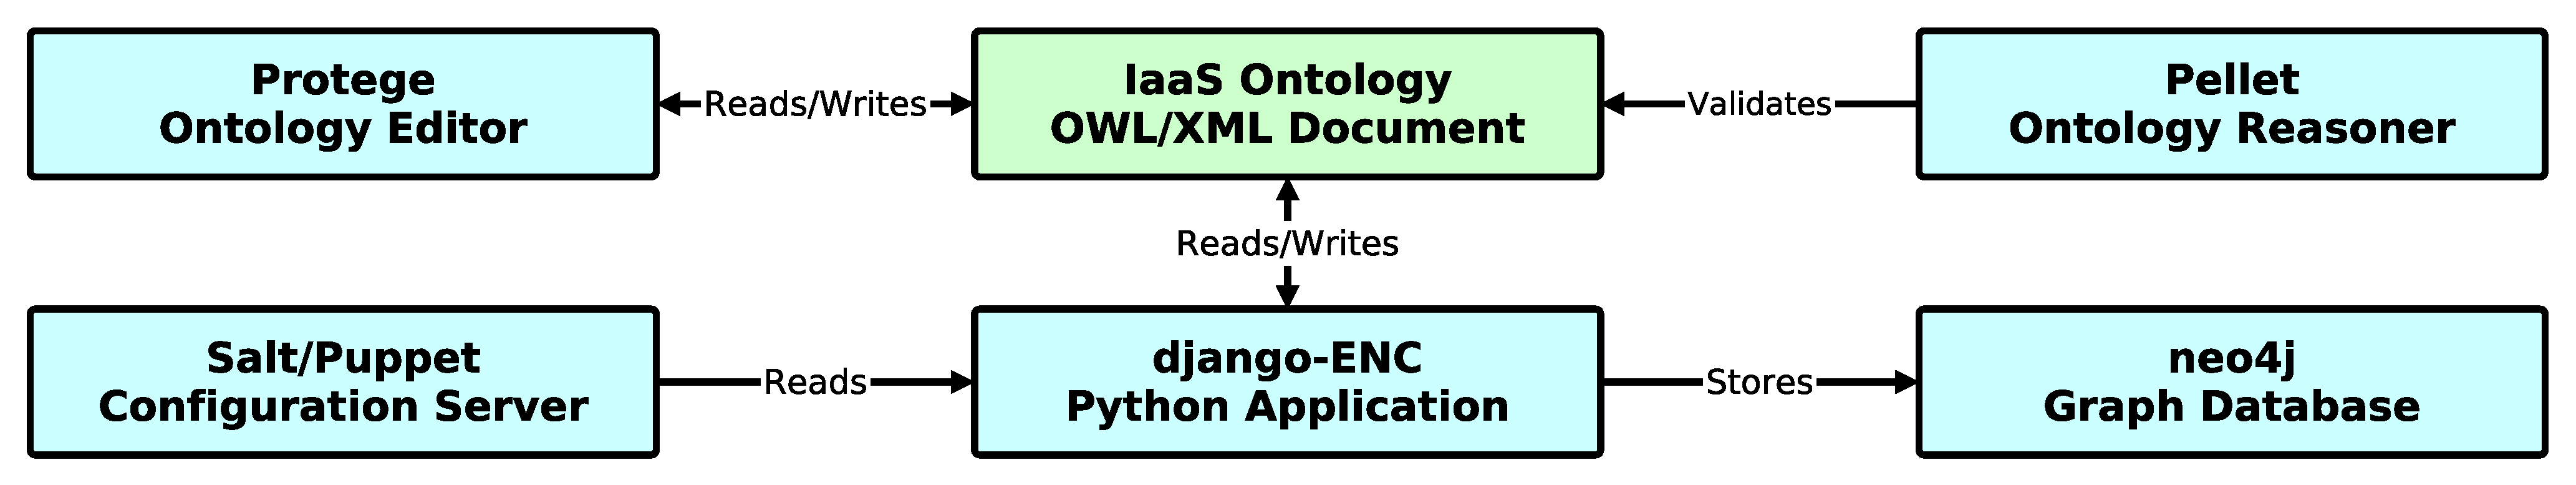
\includegraphics[scale=.17]{img/django_enc_arch.eps}
\caption{Ontology Service Architecture}
\label{fig:cm}
\end{figure}

The django-ENC service  use  web framework Django to deliver web services and asynchronous task queue Celery to perform time consuming tasks like ontology assertions and synchronizations between XML and graph database. Service expose it's owns HTTP REST API that can be consumed by configuration management tools like Salt or Puppet through their External Node Classification option.

The metada passed to CM tools is valid for 1st level of Cloud computing ontology [cite].

We have successfully tested service status enforcemet of several complete OpenStack installations by SaltStack configuration management tool with metadata acquired from Ontology ENC API.

The deployment process is not yet fully automated as there is need of setting up network and storage resources manually, but the progress in both configuration management tools and network and storage will allow better automation of these components by in-place agents or access protocols like SSH in the future.

\subsection{Samples of Ontology}

Given use case scenario Lab1 we have 3 virtual servers providing OpenStack and other core services in high-availability mode. These servers are virtualised in common. 20 physical servers  

\subsubsection{Service components of controller1}

Services located on controller server

\begin{lstlisting}
  <owl:Class rdf:about="#Glance">
    <owl:disjointWith>
      <owl:Class rdf:about="#"/>
    </owl:disjointWith>
    <owl:disjointWith>
      <owl:Class rdf:about="#ServiceInterface"/>
    </owl:disjointWith>
    <rdfs:subClassOf>
      <owl:Class rdf:about="#Composition"/>
    </rdfs:subClassOf>
  </owl:Class>
\end{lstlisting}

\subsubsection{Detail of service glance.image}

On of the services defined on the controller node is image service Glance. Following definitiong


\begin{lstlisting}
  <owl:Class rdf:about="#Glance">
    <owl:disjointWith>
      <owl:Class rdf:about="#"/>
    </owl:disjointWith>
    <owl:disjointWith>
      <owl:Class rdf:about="#ServiceInterface"/>
    </owl:disjointWith>
    <rdfs:subClassOf>
      <owl:Class rdf:about="#Composition"/>
    </rdfs:subClassOf>
    <owl:disjointWith>
      <owl:Class rdf:about="#ServiceInterface"/>
    </owl:disjointWith>
    <rdfs:subClassOf>
      <owl:Class rdf:about="#Composition"/>
    </rdfs:subClassOf>
  </owl:Class>
\end{lstlisting}

\subsubsection{Detail of data property type}

The resource can have data property and are derived mostly from Dublin Core metadata terms.

\begin{lstlisting}
  <owl:Class rdf:about="#Glance">
    <owl:disjointWith>
      <owl:Class rdf:about="#"/>
    </owl:disjointWith>
    <owl:disjointWith>
      <owl:Class rdf:about="#ServiceInterface"/>
    </owl:disjointWith>
    <rdfs:subClassOf>
      <owl:Class rdf:about="#Composition"/>
    </rdfs:subClassOf>
  </owl:Class>
\end{lstlisting}

\subsubsection{Detail of object property database}

Resources can have object property types that describe more complex relations. 

\begin{lstlisting}
  <owl:Class rdf:about="#Glance">
    <owl:disjointWith>
      <owl:Class rdf:about="#"/>
    </owl:disjointWith>
    <owl:disjointWith>
      <owl:Class rdf:about="#ServiceInterface"/>
    </owl:disjointWith>
  </owl:Class>
\end{lstlisting}
